\documentclass[12pt]{article}
\usepackage{sbc-template}
\usepackage[T1]{fontenc}
\usepackage[utf8]{inputenc}
\usepackage[brazil]{babel}
\usepackage{url}
\usepackage{graphicx}
\graphicspath{{../analysis/}{./}}
\sloppy

\title{Mineração de proxies DORA em repositórios open-source:
validade e sensibilidade das definições operacionais}
\author{Davi Érico\inst{1}, Gustavo Prehl\inst{1}, Lucas Resende\inst{1}}
\address{Engenharia de Software\\
Pontifícia Universidade Católica de Minas Gerais (PUC Minas)}
\begin{document}
\maketitle

\begin{abstract}
This study proposes mining software delivery proxies from public GitHub
repositories using GitHub Actions. Releases, commit timestamps and workflow
runs support alternative operational definitions of DORA metrics. In the 183
most popular of 300 selected repositories, the median project publishes one
release every four weeks, and lead time per release exceeds lead time per
commit (250 h versus 172 h). The two change failure rate proxies diverge
(medians 0.047 for CI failures and 0.275 for corrective releases), as do the
DORA categories: no project is Elite in frequency, while 81\% are Elite in CI
failure rate. Deployment frequency is positively correlated with both change
failure rate variants (Spearman $\rho = 0.151$ for CI failures and $0.547$ for
corrective releases), contrary to the DORA claim that speed and stability do
not compete. Language, popularity and community size show no significant
differences after Holm correction. A single-rater validation of the corrective
release heuristic on 178 releases yields precision 0.234, recall 0.929 and
F1 0.374, indicating that this proxy overestimates delivery failures.
\end{abstract}

\begin{resumo}
Este estudo propõe minerar proxies de entrega de software em repositórios
públicos do GitHub que utilizam GitHub Actions. Releases, datas de commits e
execuções de workflows sustentam definições operacionais alternativas das
métricas DORA. Nos 183 mais populares dos 300 repositórios selecionados, o
projeto mediano publica uma release a cada quatro semanas, e o lead time por
release supera o por commit (250 h contra 172 h). As duas variantes de taxa de
falha divergem (medianas de 0,047 para falhas de CI e 0,275 para releases
corretivas), assim como as categorias DORA: nenhum projeto é Elite em
frequência, enquanto 81\% são Elite em falha de CI. A frequência de deploy correlaciona-se
positivamente com as duas variantes de taxa de falha (Spearman $\rho = 0{,}151$
para falhas de CI e $0{,}547$ para releases corretivas), contrariando a
afirmação do DORA de que velocidade e estabilidade não competem. Linguagem,
popularidade e tamanho da comunidade não mostram diferenças significativas
após a correção de Holm. Uma validação com avaliador único da heurística de
release corretiva, em 178 releases, resulta em precisão 0,234, recall 0,929 e
F1 0,374, o que indica que esse proxy superestima as falhas de entrega.
\end{resumo}

\section{Introdução}
\label{sec:introducao}

A entrega frequente de mudanças precisa ser analisada em conjunto com a
estabilidade do software. O trabalho de Forsgren, Humble e Kim
\cite{accelerate} e as métricas de desempenho de entrega do DORA \cite{dora}
motivam o estudo dessa relação. Neste laboratório, o interesse recai sobre
frequência de entrega, tempo entre a escrita e a entrega de mudanças,
proporção de entregas com falha e tempo de recuperação. Adotam-se as quatro
dimensões e os cortes de classificação fixados pelo enunciado, preservando
definições comuns entre os grupos da disciplina.

Repositórios públicos oferecem releases, commits e registros de integração
contínua, mas esses registros não demonstram, por si só, quando uma mudança
chegou à produção ou provocou um incidente. Uma release de biblioteca pode
ser disponibilizada sem adoção imediata; uma falha de CI pode impedir uma
entrega em vez de representar falha em produção. Os valores minerados são,
portanto, \textit{proxies}, cujo significado depende de suas definições
operacionais.

O objetivo deste estudo é caracterizar proxies DORA em projetos open-source
que utilizam GitHub Actions e avaliar a confiança nas comparações resultantes.
As questões de pesquisa investigam frequência de releases (RQ01), lead time
(RQ02), taxas de falha (RQ03), recuperação de workflows (RQ04), associação
entre frequência e falha (RQ05), diferenças entre características dos projetos
(RQ06) e sensibilidade da classificação às definições operacionais (RQ07).

O protocolo da disciplina prevê uma janela de doze meses, uma amostra final
de pelo menos 300 repositórios elegíveis e definições comuns. São elegíveis
projetos públicos com mais de 1.000 estrelas, pelo menos cinco releases
publicadas e 50 execuções válidas de GitHub Actions no branch padrão durante
a janela. Para lead time,
serão comparadas a mediana dos tempos por release, considerando o commit
mais antigo de cada entrega, e a mediana dos tempos de todos os commits
incluídos nas releases. A paginação da API evita que essas comparações sejam
limitadas silenciosamente a uma fração dos commits \cite{github}.

A janela adotada para a S02 abrange 6 de outubro de 2025 a 7 de outubro de
2026, à meia-noite no fuso UTC$-3$, com o limite final exclusivo. São 366 dias,
um dia além dos doze meses previstos. A exceção foi autorizada por Gustavo em
13 de outubro de 2026, após a coleta parcial, para compatibilidade com os
183 repositórios informados pelo outro integrante. A confirmação docente
registrada na main em 14 de outubro refere-se à janela original de doze
meses; a aprovação da extensão de um dia não está registrada. A configuração
versionada distingue essas decisões; eventual revisão exigirá revalidar os
dados e repetir a coleta quando necessário. O piloto inicial previa 100
repositórios elegíveis, mas seu manifesto registra execução interrompida.
Esta versão relata os resultados das RQ05 e RQ06 e a validação parcial do CFR
(b) sobre os 300 repositórios do dataset congelado. As demais questões estão
marcadas como pendentes na seção de resultados.

O protocolo previa examinar a validade dos proxies com três avaliadores
independentes em 60 repositórios, com cinco releases por projeto, e medir a
concordância e a qualidade da heurística corretiva contra o consenso. Por
decisão do grupo, apenas um avaliador humano rotulou a amostra-ouro. A
validação do CFR (b) foi feita, portanto, com um único avaliador, e esse
desvio é discutido na Seção~\ref{sec:validacao-cfrb}. A comparação entre
combinações de releases, pré-releases, tags e variantes de lead time e CFR
avaliará a estabilidade das classificações.

\subsection{Hipóteses a priori}

As hipóteses abaixo acompanham o protocolo versionado antes da coleta deste
estudo; a revisão conjunta permanece pendente. Elas expressam expectativas
a confrontar com os dados, não resultados observados. Revisões posteriores
à observação dos resultados deverão ser identificadas como exploratórias.

\begin{description}
\item[H01 (RQ01).] Espera-se heterogeneidade na frequência de releases,
com concentração abaixo de uma entrega semanal, pois projetos podem
agrupar mudanças em ciclos distintos de publicação.
\item[H02 (RQ02).] Espera-se que a variante por release apresente, em geral,
lead times superiores aos da variante por commit, pela influência de commits
antigos. Não é uma identidade matemática: as variantes ponderam as releases
de formas diferentes.
\item[H03 (RQ03).] Espera-se divergência entre CFR baseado em CI e baseado
em releases corretivas, pois capturam eventos distintos. Não se antecipa
ordenação obrigatória entre seus valores.
\item[H04 (RQ04).] Espera-se distribuição assimétrica dos tempos de
recuperação, com muitos episódios curtos e alguns prolongados. Episódios
não encerrados durante a janela deverão permanecer registrados como censurados.
\item[H05 (RQ05).] Espera-se associação monotônica fraca ou não positiva
entre frequência e CFR. Spearman será calculado para ambas as variantes
de CFR, sem interpretar associação como causalidade.
\item[H06 (RQ06).] Espera-se diferença entre subgrupos em pelo menos uma
métrica. O protocolo fixa linguagem principal, quartis de estrelas e quartis
de contribuidores como fatores antes de observar resultados.
\item[H07 (RQ07).] Espera-se que parte dos repositórios mude de categoria
DORA ao alterar as definições de entrega, lead time e CFR, especialmente
próximo aos cortes de classificação.
\end{description}

Os artefatos serão organizados em módulos de coleta, normalização, métricas e
análise, com testes e rastreabilidade por issues. Validação manual, sensibilidade
e replicação cruzada deverão sustentar a discussão dos limites do estudo.
Repositório: \url{https://github.com/lucasrsnd/lab-medicao-experimentacao}.
Acompanhamento: \url{https://github.com/users/lucasrsnd/projects/2}.

% Metodologia. Fonte das decisões: Lab-03/docs/protocolo.md e config/estudo.json.
\section{Metodologia}
\label{sec:metodologia}

\subsection{População, seleção e amostra analisada}
\label{sec:amostra}

A população-alvo são repositórios públicos do GitHub com mais de 1.000
estrelas que usam GitHub Actions. A busca \texttt{stars:>1000}, ordenada por
estrelas, informou 65.512 repositórios. Os 1.800 mais populares formaram a
lista de candidatos. Destes, 1.563 usam Actions. São elegíveis os que têm, na
janela, pelo menos cinco releases publicadas no histórico do branch padrão e
pelo menos 50 workflow runs válidos disparados por \texttt{push} nesse branch.
Para limitar o custo da coleta, também ficaram de fora repositórios com mais de
500 releases ou mais de 1.000 runs de \texttt{push} na janela. Restaram 311
elegíveis, e os 300 mais populares formaram a seleção. A amostra é intencional
(por popularidade), não aleatória.

A coleta foi dividida nos índices 0--182 e 183--299. Na segunda parte, 17
repositórios não cumpriram o mínimo de releases na verificação de ancestralidade
e foram substituídos pelos próximos elegíveis em ordem de estrelas
(\texttt{data/selecao-amostra-revisada.json}).

\textbf{Amostra analisada.} O dataset congelado
(\texttt{data/amostra\_completa.json.gz}, coleta de 13 de outubro de 2026)
reúne 183 e 117 repositórios, totalizando os 300 selecionados. A janela e os
critérios são comuns às partes; todos usam a heurística v2. A amostra varia de
cerca de 24 mil a 289 mil estrelas e não representa projetos menos populares.

\subsection{Janela e unidades}

A janela vai de 6 de outubro de 2025 a 7 de outubro de 2026 (UTC$-3$), com fim
exclusivo, e tem 366 dias. O dia além dos doze meses é uma exceção de
compatibilidade, discutida na introdução. Releases e runs entram pela data de
publicação e de criação, respectivamente. Commits incluídos em releases da
janela podem ser anteriores a ela.

\subsection{Métricas}

\textbf{Frequência (RQ01):} releases publicadas na janela divididas pela sua
duração em semanas. \textbf{Lead time (RQ02):} cada release é comparada com a
anterior. A variante (a) é a mediana, por repositório, do intervalo entre a
publicação e o commit mais antigo da release. A variante (b) é a mediana sobre
todos os commits incluídos. \textbf{CFR (RQ03):} a variante (a) é a proporção de
runs de CI com falha entre os runs com sucesso ou falha. A variante (b) é a
proporção de releases seguidas, em até sete dias, por uma release corretiva.
Releases dos últimos sete dias da janela são censuradas. A heurística v2
considera corretiva a release que só altera o \textit{patch} semver, ou em que
pelo menos metade dos commits cita \texttt{revert}, \texttt{hotfix} ou
\texttt{fix}. \textbf{Recuperação (RQ04):} horas entre o início da primeira
falha e o próximo sucesso no mesmo workflow. Episódios abertos no fim da
janela são censurados.

A classificação DORA usa os cortes do enunciado. A categoria geral é a mediana
das quatro notas (Elite~4 a Low~1), arredondada para baixo, e só é emitida
quando as quatro métricas são observadas. A configuração de referência C1 usa
releases publicadas, lead time (a) e CFR (a). As configurações C2 (com
pré-releases, lead time (b) e CFR (b)) e C3 (tags) servem à RQ07. Ausências
nunca são imputadas como zero, e cada uma tem o motivo registrado.

\subsection{Validação manual}

O protocolo previa 60 repositórios, cinco releases por projeto e rotulagem
cega por três avaliadores. O relatório disponível cobre 283 releases em 58
repositórios, mas seu hash de origem difere do dataset congelado; os resultados
não validam diretamente o CFR (b) dos 300 repositórios. Só um avaliador humano
concluiu a rotulagem, sem consenso (Seção~\ref{sec:validacao-cfrb}).

\subsection{Análise estatística}

As métricas são descritas por mediana e IQR. A RQ05 usa a correlação de
Spearman entre a frequência e cada CFR. A RQ06 usa Kruskal-Wallis, com
$\varepsilon^2$ como tamanho de efeito, para linguagem principal e quartis de
estrelas e de contribuidores, fatores fixados antes da coleta. Comparações
múltiplas são corrigidas por Holm ($\alpha = 0{,}05$). A RQ07 compara as
classificações por percentual de mudança de categoria e kappa de Cohen
ponderado linear. Todas as análises são reexecutáveis a partir do dataset
congelado (\texttt{python -m lab03.analysis.*}).

% Resultados por RQ (S03-08, #127). Valores gerados por `python -m lab03.analysis.*`
% a partir de analysis/base_repositorios.csv; ver Lab-03/analysis/README.md.
\providecommand{\pendente}[1]{\textbf{[Pendente: #1]}}

\section{Resultados}

Os resultados abaixo usam os 300 repositórios do dataset congelado
(\texttt{data/amostra\_completa.json.gz}), achatados em uma linha por
repositório (\texttt{analysis/base\_repositorios.csv}). Seguindo o protocolo,
reportam-se mediana e IQR. Métricas ausentes não são imputadas, e por isso o
$n$ varia por análise. Toda correção para comparações múltiplas usa Holm, com
$\alpha = 0{,}05$.

\subsection{RQ01 a RQ04: métricas DORA}

A Tabela~\ref{tab:rq01-rq04} resume as quatro métricas por repositório. O $n$
válido varia porque 11 repositórios não têm release avaliável para lead time e
CFR (b), e 32 não têm episódio de recuperação encerrado.

\begin{table}[ht]
\centering
\caption{RQ01--RQ04: distribuição por repositório. Fontes:
\texttt{analysis/rq01\_rq02/} e \texttt{analysis/rq03\_rq04/}
(\texttt{lab03.analysis.rq01\_rq02}, \texttt{lab03.analysis.rq03\_rq04}).}
\label{tab:rq01-rq04}
\small
\begin{tabular}{lrrr}
\hline
Métrica & $n$ & Mediana & [Q1--Q3] \\
\hline
Frequência (releases/semana) & 300 & 0,268 & [0,134--0,555] \\
Lead time (a), por release (h) & 289 & 250,8 & [70,3--756,5] \\
Lead time (b), por commit (h) & 289 & 169,4 & [53,9--546,0] \\
CFR (a), runs de CI com falha & 300 & 0,054 & [0,020--0,142] \\
CFR (b), release corretiva em 7 dias & 289 & 0,292 & [0,125--0,522] \\
Recuperação (h) & 268 & 4,89 & [0,84--21,48] \\
\hline
\end{tabular}
\end{table}

\textbf{RQ01.} A mediana é de uma release a cada quatro semanas, e 266 dos 300
repositórios (89\%) publicam menos de uma por semana, o que sustenta a H01.
Nove repositórios não publicaram release na janela.

\textbf{RQ02.} O lead time por release supera o por commit nas medianas (250,8
h contra 169,4 h) e em 212 dos 289 repositórios (73\%), como previa a H02. A
variante (a) dá peso a cada release e cresce quando uma entrega inclui um
commit antigo, enquanto a (b) dilui esse commit entre os demais
(Figura~\ref{fig:rq01-rq02}).

\begin{figure}[ht]
\centering
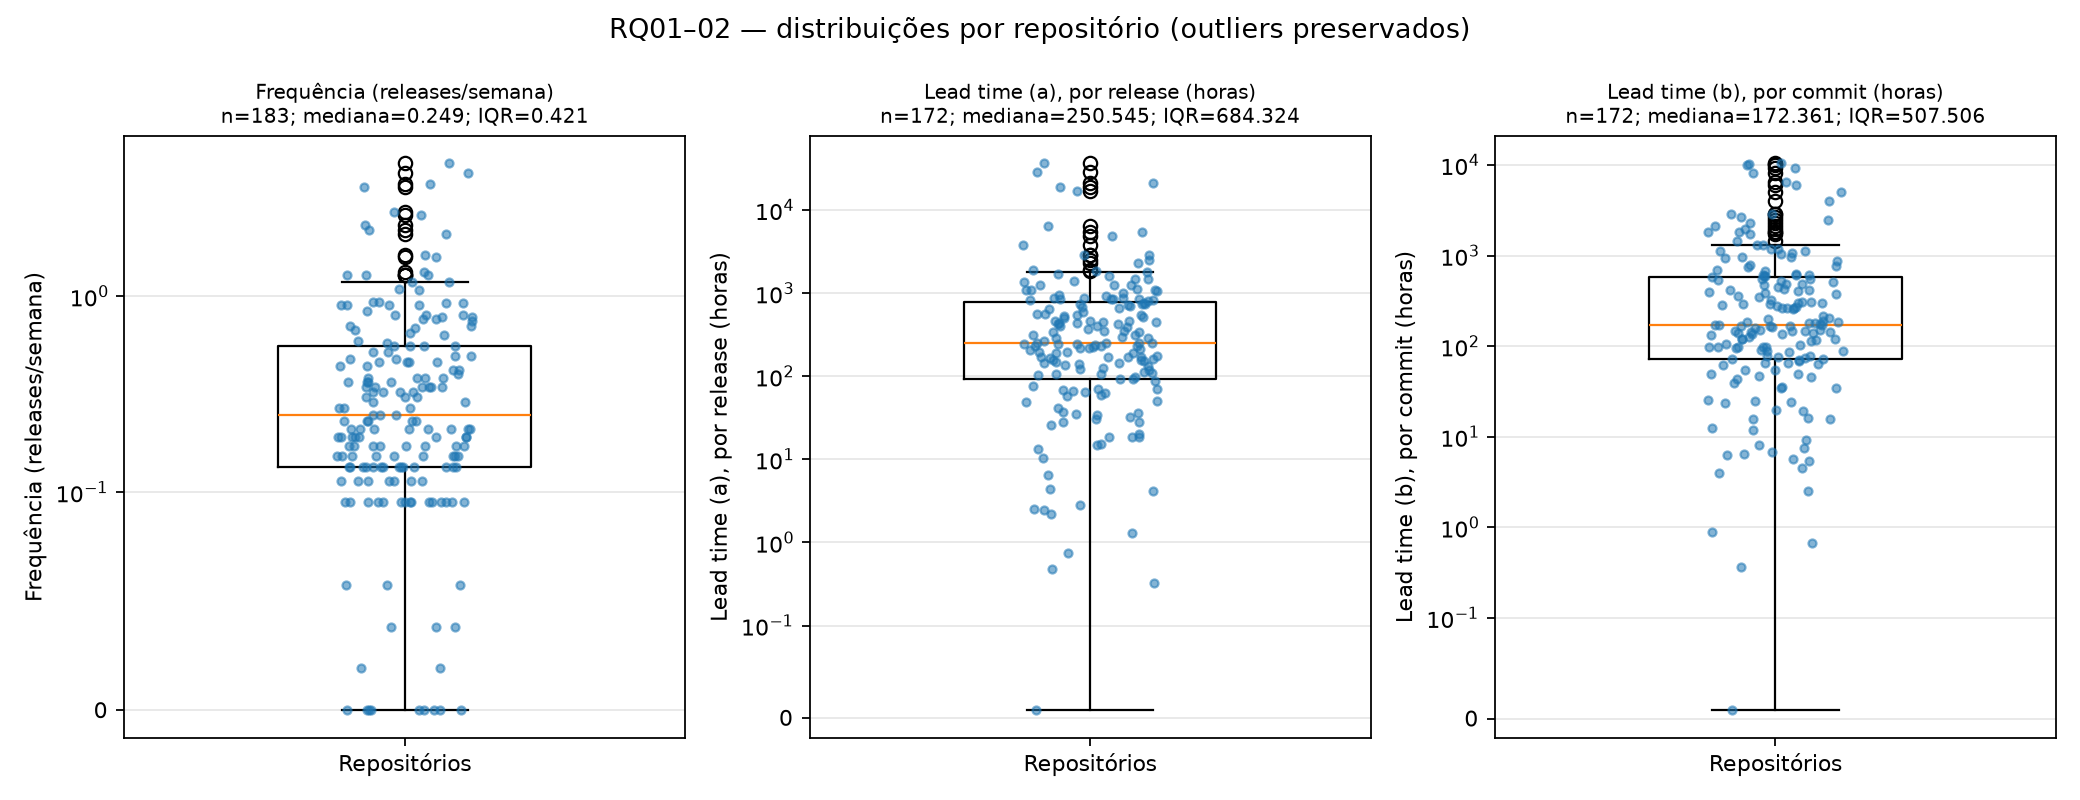
\includegraphics[width=\textwidth]{rq01_rq02/rq01_rq02_distribuicoes.png}
\caption{RQ01--RQ02: distribuições de frequência e lead time (a) e (b), em
escala \textit{symlog}, com todos os outliers preservados.}
\label{fig:rq01-rq02}
\end{figure}

\textbf{RQ03.} As duas variantes de CFR divergem, como previa a H03. Nos 289
repositórios com ambas, a mediana da diferença CFR (b) $-$ CFR (a) é 0,200 (IQR
0,409), com o CFR (b) mais de cinco vezes maior nas medianas
(Figura~\ref{fig:rq03}). Parte dessa distância vem da própria heurística: a
validação parcial (Seção~\ref{sec:validacao-cfrb}) indica que o CFR (b)
superestima as releases corretivas. Nenhuma das duas variantes observa falha em
produção.

\begin{figure}[ht]
\centering
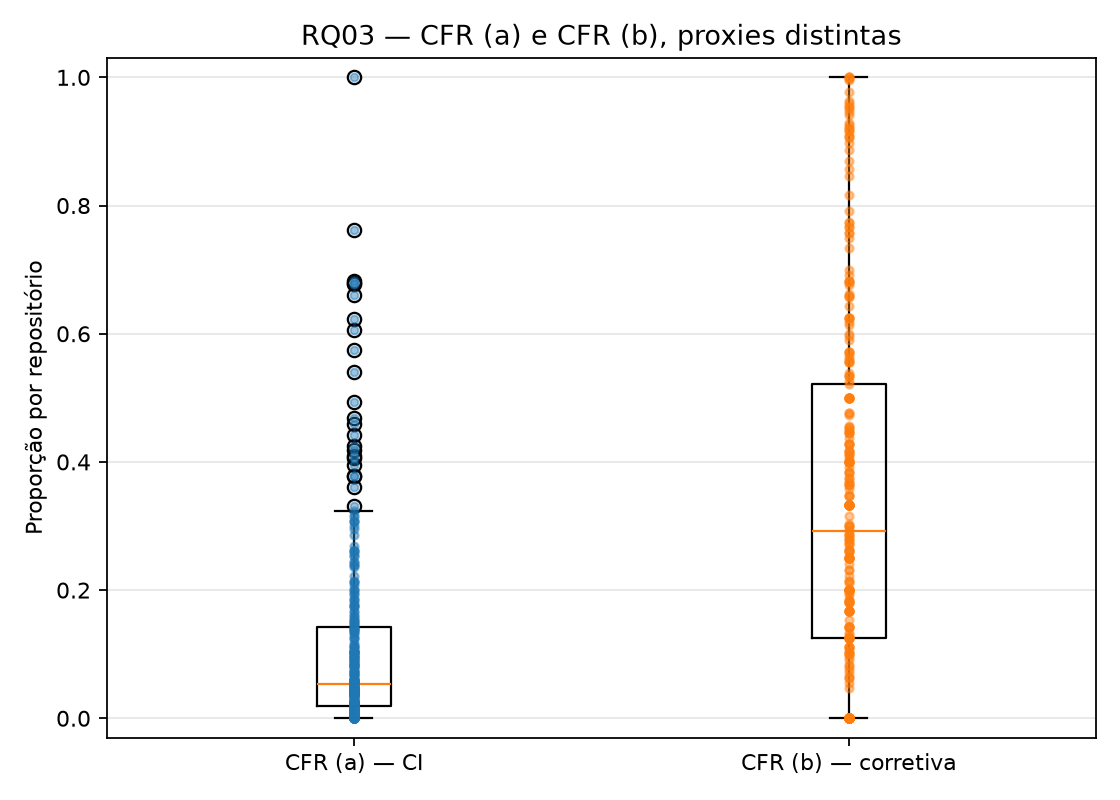
\includegraphics[width=0.7\textwidth]{rq03_rq04/rq03_cfr_comparacao.png}
\caption{RQ03: comparação entre CFR (a) e CFR (b) por repositório.}
\label{fig:rq03}
\end{figure}

\textbf{RQ04.} A recuperação é assimétrica, como previa a H04: mediana de 4,9 h,
com terceiro quartil de 21,5 h. Dos 4.119 episódios, 75 (1,8\%) não foram
encerrados na janela. Eles foram mantidos como censurados, sem tempo imputado.
No CFR (b), 251 das 8.518 releases (2,9\%) são censuradas por não terem os sete
dias seguintes inteiros na janela.

A Tabela~\ref{tab:c1} mostra a classificação DORA de referência (C1), com os
cortes do enunciado. A categoria geral é a mediana das quatro pontuações,
arredondada para baixo, e só é emitida quando as quatro métricas são
observadas. Por isso 40 repositórios ficam sem categoria geral.

\begin{table}[ht]
\centering
\caption{Classificação DORA C1 por métrica e geral (300 repositórios). Fonte:
\texttt{analysis/c1\_reference/c1\_resultados.json}
(\texttt{lab03.analysis.c1\_reference}).}
\label{tab:c1}
\small
\begin{tabular}{lrrrrr}
\hline
Métrica & Elite & High & Medium & Low & Não classif. \\
\hline
Frequência & 0 & 34 & 130 & 136 & 0 \\
Lead time (a) & 42 & 72 & 98 & 77 & 11 \\
CFR (a) & 230 & 40 & 17 & 13 & 0 \\
Recuperação & 77 & 135 & 40 & 16 & 32 \\
Geral & 17 & 89 & 130 & 24 & 40 \\
\hline
\end{tabular}
\end{table}

Os proxies colocam os projetos em pontos opostos da escala: nenhum é Elite em
frequência, e 45\% são Low, enquanto 77\% são Elite em CFR (a). A categoria
geral concentra-se em Medium e High. Como a C1 usa o CFR (a), o efeito de
trocar pela variante (b), que é bem maior, é tema da RQ07.

\subsection{RQ05: frequência de deploy e taxa de falha}

A Tabela~\ref{tab:rq05} apresenta a correlação de Spearman entre a frequência
de deploy e cada variante de CFR, com $n$ pareado (repositórios com as duas
métricas). As duas associações são positivas: repositórios que publicam mais
releases têm, em postos, CFR \emph{maior}. A associação com o CFR (a), de CI, é
fraca, mas significativa ($\rho = 0{,}182$; $p_{Holm} = 0{,}002$). Com o CFR
(b), de release corretiva, ela é forte ($\rho = 0{,}567$; $p_{Holm} <
0{,}001$). A Figura~\ref{fig:rq05} mostra as dispersões.

\begin{table}[ht]
\centering
\caption{RQ05: Spearman entre frequência (releases/semana) e CFR. Fonte:
\texttt{analysis/rq05/rq05\_resultados.json} (\texttt{lab03.analysis.rq05}).}
\label{tab:rq05}
\small
\begin{tabular}{lrrrrc}
\hline
Variante de CFR & $n$ & CFR mediano [IQR] & $\rho$ & $p_{Holm}$ & CFR $= 0$ \\
\hline
(a) runs de CI com falha & 300 & 0,054 [0,020--0,142] & 0,182 & 0,002 & 24 \\
(b) release corretiva em 7 dias & 289 & 0,292 [0,125--0,522] & 0,567 & $1{,}1\times10^{-25}$ & 52 \\
\hline
\end{tabular}
\end{table}

\begin{figure}[ht]
\centering
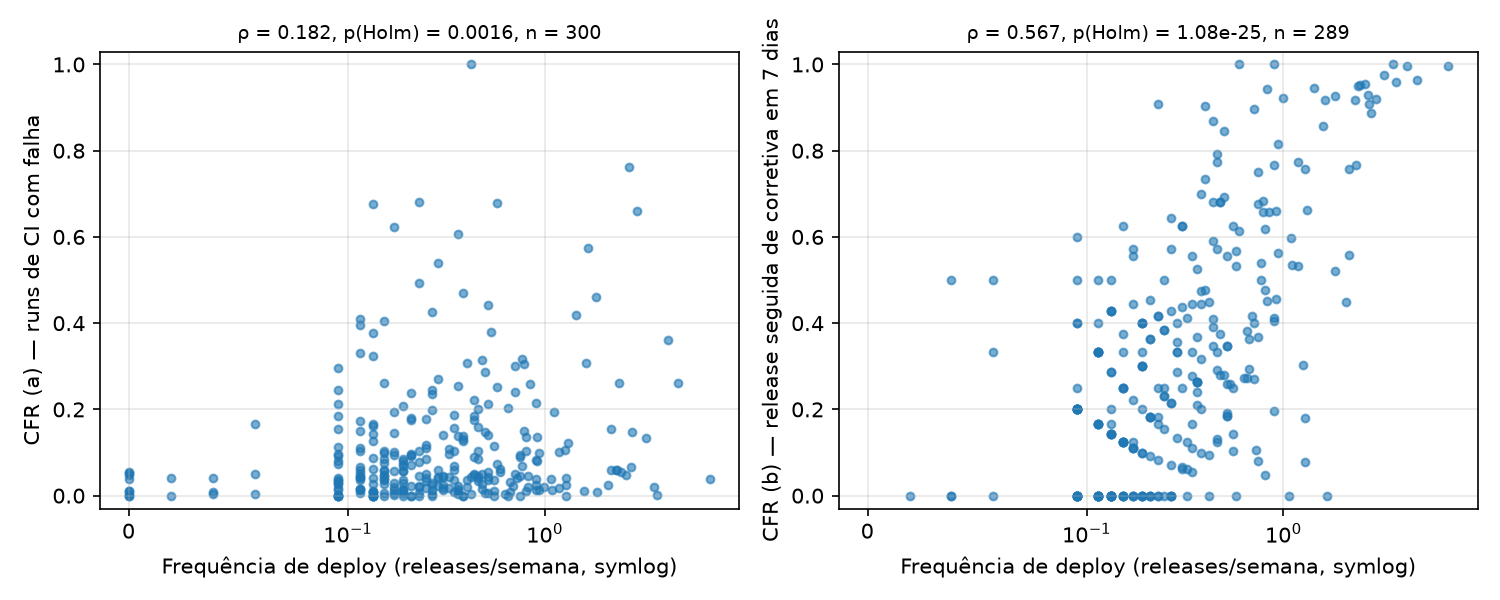
\includegraphics[width=\textwidth]{rq05/rq05_dispersao.png}
\caption{RQ05: frequência de deploy (eixo X em escala \textit{symlog}, que
mantém os 9 repositórios sem release na janela) versus CFR (a) e CFR (b).}
\label{fig:rq05}
\end{figure}

Nenhuma das variantes sustenta a afirmação do DORA de que velocidade e
estabilidade não competem, o que exigiria $\rho$ negativo. A magnitude no CFR
(b) é em parte induzida pela definição: com mais releases por semana, é mais
provável que uma release \textit{patch} ocorra nos sete dias seguintes e seja
marcada como corretiva. O CFR (a), que mede falha de pipeline e independe do
ritmo de releases, mostra associação fraca. Em ambos os casos trata-se de
associação monotônica, sem implicação causal: tamanho e atividade do projeto,
por exemplo, podem elevar as duas métricas. A validação parcial da heurística
(Seção~\ref{sec:validacao-cfrb}) indica ainda que o CFR (b) superestima as
releases corretivas, o que reforça a cautela com essa associação.

\subsection{RQ06: características dos repositórios}

Os fatores pré-registrados são linguagem principal (TypeScript 77, Python 60,
``Outras'' 51, que reúne as 16 linguagens com menos de 10 repositórios, Go 31,
JavaScript 31, Rust 25, C++ 13 e Java 10), quartis de estrelas (75 por quartil)
e quartis de contribuidores (74 a 76 por quartil). Dois repositórios não têm
linguagem principal. As métricas são as da configuração de referência C1. A
Tabela~\ref{tab:rq06} resume os 12 testes de Kruskal-Wallis, com tamanho de
efeito $\varepsilon^2 = H/(n-1)$.

\begin{table}[ht]
\centering
\caption{RQ06: Kruskal-Wallis por fator e métrica (C1). Células: $\varepsilon^2$
($p_{Holm}$); * indica significância após Holm. Fonte:
\texttt{analysis/rq06/rq06\_resultados.json} (\texttt{lab03.analysis.rq06}).}
\label{tab:rq06}
\small
\begin{tabular}{lcccc}
\hline
Fator & Frequência & Lead time (a) & CFR (a) & Recuperação \
 & $n = 300$ & $n = 289$ & $n = 300$ & $n = 268$ \
\hline
Linguagem ($k = 8$) & 0,055 (0,22) & 0,099 (0,002)* & 0,041 (0,82) & 0,027 (1,00) \
Estrelas ($k = 4$) & 0,010 (1,00) & 0,002 (1,00) & 0,022 (0,82) & 0,011 (1,00) \
Contribuidores ($k = 4$) & 0,007 (1,00) & 0,053 (0,017)* & 0,001 (1,00) & 0,017 (1,00) \
\hline
\end{tabular}
\end{table}

Dois dos 12 testes são significativos após a correção de Holm, ambos sobre o
lead time (a). Por linguagem, $H = 28{,}37$ ($p_{Holm} = 0{,}002$;
$\varepsilon^2 = 0{,}099$, médio): as medianas vão de 163~h em TypeScript e
181~h em Python a 565~h em Rust e 1.070~h em C++ (12 repositórios). Por quartil
de contribuidores, $H = 15{,}35$ ($p_{Holm} = 0{,}017$; $\varepsilon^2 =
0{,}053$, pequeno): a mediana é de 142~h e 157~h nos dois primeiros quartis e de
416~h e 403~h nos dois últimos, o que sugere entregas mais espaçadas em projetos
com mais colaboradores. Frequência, CFR (a), recuperação e estrelas não
diferem de forma significativa, e os efeitos nessas combinações são
desprezíveis ou pequenos ($\varepsilon^2 \le 0{,}055$). Os testes não indicam
quais grupos diferem entre si, pois não houve comparações \textit{post hoc}.
Linguagem e número de contribuidores podem refletir o tipo de projeto (por
exemplo, bibliotecas de sistemas contra aplicações web), que não foi
controlado. Como alguns grupos têm 10 a 13 repositórios, os resultados por
linguagem são menos estáveis. Medianas e IQR por grupo estão em
\texttt{analysis/rq06/rq06\_grupos.csv}. O tipo de projeto não foi usado como
fator, porque só está rotulado para os 60 repositórios da amostra-ouro.

\subsection{Validação do CFR (b): avaliador único}
\label{sec:validacao-cfrb}

O protocolo previa três avaliadores independentes e consenso sobre 300
releases. Isso não foi cumprido: por decisão do grupo, a segunda rodada
(\texttt{labels/reamostragem-v2/}) não foi rotulada, e na primeira rodada só um
integrante (avaliador B) rotulou as releases. Os rótulos do avaliador A são
rascunhos gerados por IA, marcados como tal em todas as linhas. Por isso não
há consenso nem medida de confiabilidade entre avaliadores. O resultado a
seguir é uma \emph{validação de avaliador único} e não o F1 contra consenso
previsto no protocolo.

A primeira rodada foi sorteada da mesma coleta do snapshot (13 de outubro de
2026, mesma janela). Com o dataset de 300 repositórios, todas as 283 releases
sorteadas, em 58 repositórios, constam do snapshot e têm identificador e
veredito da heurística conferidos, e nenhuma foi excluída. A
Tabela~\ref{tab:validacao-cfrb} compara a heurística v2 com os rótulos de B.

\begin{table}[ht]
\centering
\caption{CFR (b): heurística v2 × avaliador B (283 releases, 58 repositórios).
IC 95\% de Wilson. Fonte: \texttt{analysis/validacao\_cfr\_b/resultados.json}
(\texttt{lab03.analysis.cfr\_b\_validation}).}
\label{tab:validacao-cfrb}
\small
\begin{tabular}{lrr|lr}
\hline
B $\backslash$ heurística & não & sim & Métrica & Valor [IC 95\%] \\
\hline
não & 109 & 128 & Precisão & 0,238 [0,180--0,308] \\
sim & 6 & 40 & Recall & 0,870 [0,743--0,939] \\
 & & & F1 & 0,374 \\
\hline
\end{tabular}
\end{table}

A heurística deixa escapar poucas releases corretivas (6 de 46), mas só 40
das 168 releases que ela marca como corretivas foram confirmadas por B. O F1
fica bem abaixo do limiar de 0,70 do protocolo. O CFR (b) deve, portanto, ser
lido como tendendo a superestimar a taxa de falha. Uma explicação plausível,
ainda não verificada caso a caso, são as releases \textit{patch} publicadas em
até sete dias sem corrigir a entrega anterior.
Como referência auxiliar, e não como segundo avaliador, os rascunhos de IA
concordam com B em 88\% das releases ($\kappa$ de Cohen $= 0{,}590$). Os
intervalos tratam as releases como independentes, embora venham agrupadas em
cinco por repositório, e por isso são otimistas. Com um único avaliador, erros
ou critérios pessoais de B não podem ser separados do erro da heurística.

\subsection{RQ07: sensibilidade da classificação}

Comparando a categoria geral entre as variantes, há mudança em todos os pares
(Tabela~\ref{tab:rq07}). Só entram repositórios classificados nas duas
variantes; os demais são excluídos, sem imputação. O kappa de Cohen usa pesos
lineares para a ordem Low $<$ Medium $<$ High $<$ Elite.

\begin{table}[ht]
\centering
\caption{RQ07: mudanças de categoria geral e concordância entre variantes
(300 repositórios). Fonte: \texttt{analysis/rq07/rq07\_resultados.md}
(\texttt{lab03.analysis.rq07}).}
\label{tab:rq07}
\small
\begin{tabular}{lrrrrrr}
\hline
Par & $n$ & Excluídos & Mudaram (\%) & Subiram & Desceram & $\kappa$ linear \\
\hline
C1$\times$C2 & 259 & 41 & 115 (44,4\%) & 36 & 79 & 0,311 \\
C1$\times$C3 & 260 & 40 & 74 (28,5\%) & 59 & 15 & 0,625 \\
C2$\times$C3 & 261 & 39 & 107 (41,0\%) & 99 & 8 & 0,428 \\
\hline
\end{tabular}
\end{table}

Nas exclusões, 38 repositórios não têm categoria em nenhuma variante em cada
par; além deles, C1$\times$C2 exclui 2 sem C1 e 1 sem C2, C1$\times$C3 exclui
4 sem C1, e C2$\times$C3 exclui 3 sem C2. A C3 não tem exclusões isoladas.
As mudanças que envolvem C2 exigem cautela: ela usa o CFR (b), cuja validação
de avaliador único obteve F1 = 0,374, abaixo do limiar de 0,70. Portanto, parte
das diferenças pode refletir erro da heurística, não apenas a definição de
entrega. Os resultados descrevem esta amostra e não implicam causalidade.

\begin{thebibliography}{9}
\bibitem[Forsgren et al. 2018]{accelerate}
Forsgren, N.; Humble, J.; Kim, G. (2018).
\textit{Accelerate: The Science of Lean Software and DevOps}.
IT Revolution Press.
\bibitem[DORA 2026]{dora}
DORA. \textit{DORA's software delivery performance metrics}.
Disponível em: \url{https://dora.dev/guides/dora-metrics/}.
Acesso em: 7 out. 2026.
\bibitem[GitHub 2026]{github}
GitHub. \textit{REST API endpoints for commits}.
Disponível em: \url{https://docs.github.com/en/rest/commits/commits}.
Acesso em: 7 out. 2026.
\end{thebibliography}
\end{document}
